In this section, we describe the plugin-based architecture of BrainScape's framework, designed to systematically 
collect, standardize, and preprocess anatomical MRI data. We discuss its modular structure by explaining 
the functions and interdependencies of each module.


\subsection{Overall Framework Design}

The BrainScape framework is developed in Python and employs a configurable plugin-based architecture to allow flexible 
substitution of plugins without updating the codebase. 
Each core operation, such as dataset downloading, file mapping and preprocessing is encapsulated in an independent plugin that can be configured or replaced at runtime.
Meanwhile, the BrainScape dataset includes a curated set of dataset-specific configuration files for \NumDatasets\ diverse datasets, 
each specifying the combination of downloader, mapper, and preprocessing plugins required for a given dataset, along with all necessary parameter settings.
This design allows datasets with diverse sources, file structures, and acquisition protocols to be seamlessly integrated into a unified workflow.

Each plugin is responsible for a specific task, such as downloading MRI data from a given repository, 
performing MRI preprocessing, or mapping the downloaded files to a standardized JSON record (Figure~\ref{fig:SystemArchitecture}).
Every pipeline stage (downloading, mapping, and preprocessing) has an associated abstract base class that exposes a minimal, stage-specific API 
(e.g., download(), map(), or preprocess()).
Concrete implementations such as ``OpenNeuroDownloader'' and ``SynapseDownloader'' inherit from the ``DownloaderPlugin'' base class and override these methods. 
Plugins for each stage are organized into dedicated directories, containing the base class and its associated plugins; 
For instance, all downloader plugins reside in ``download/downloader/'' alongside the downloader base class.

At run time, BrainScape employs a ``PluginLoader'' for dynamic class loading.
At the start of every workflow stage, the plugin loader scans the designated directories 
and registers each available plugin under its declared name.
(e.g., ``OpenNeuroDownloader'' or ``SynapseDownloader'' for downloader plugins).
When the workflow enters a particular stage, it consults the dataset-specific JSON configuration, 
instantiates the plugin whose declared name matches the configuration entry, passes the relevant parameters, 
and invokes the plugin's API method. 
Plugin selection is performed independently for each dataset 
and is driven entirely by its dataset-specific configuration, 
so introducing or switching plugins requires no changes to the core code.

This architecture makes the BrainScape framework intrinsically extensible. Adding a new plugin
is as simple as creating a Python file that inherits the appropriate base class 
and placing it in the correct plugin directory. 
The new plugin will then be discovered automatically, and 
researchers can easily swap out or introduce new plugins (e.g., new preprocessing pipelines) 
customized to meet their specific research needs.
Key objectives of the BrainScape framework include: 
\begin{description}
    \item[Automation:] Minimizing manual labor by automating dataset downloads, file mapping and organization, demographics attachment, and data preprocessing in a single pipeline.
    \item[Standardization:] Maintaining a common mapping record and a standardized preprocessing pipeline across all datasets, while allowing users the flexibility to incorporate dataset-specific preprocessing or other customized plugins as needed.
    \item[Extensibility:] Facilitating seamless integration of new data sources, additional preprocessing pipelines, and integration of new modules or plugins. 
    \item[Reproducibility:] Ensuring consistent execution and traceability by recording dataset-specific download, mapping, and processing parameters in JSON configuration files, thus facilitating accurate and reliable replication of the workflow.
\end{description}


\subsection{Plugin-Based Architecture}

Figure~\ref{fig:SystemArchitecture} illustrates the architecture of the BrainScape framework. 
At the core of this framework is a pipeline workflow that handles the sequential execution of the modules, 
such as downloading, mapping, and preprocessing (depicted by the red arrows in Figure~\ref{fig:SystemArchitecture}). 
This framework allows flexible selection and configuration of the plugins for each step, which can be tailored for 
each dataset via specific configuration files.
The Configurations integrate both default settings and dataset-specific overrides, maintaining consistency 
across datasets while allowing the flexibility to customize the pipeline for each dataset individually.

\begin{figure}[htbp]\begin{center}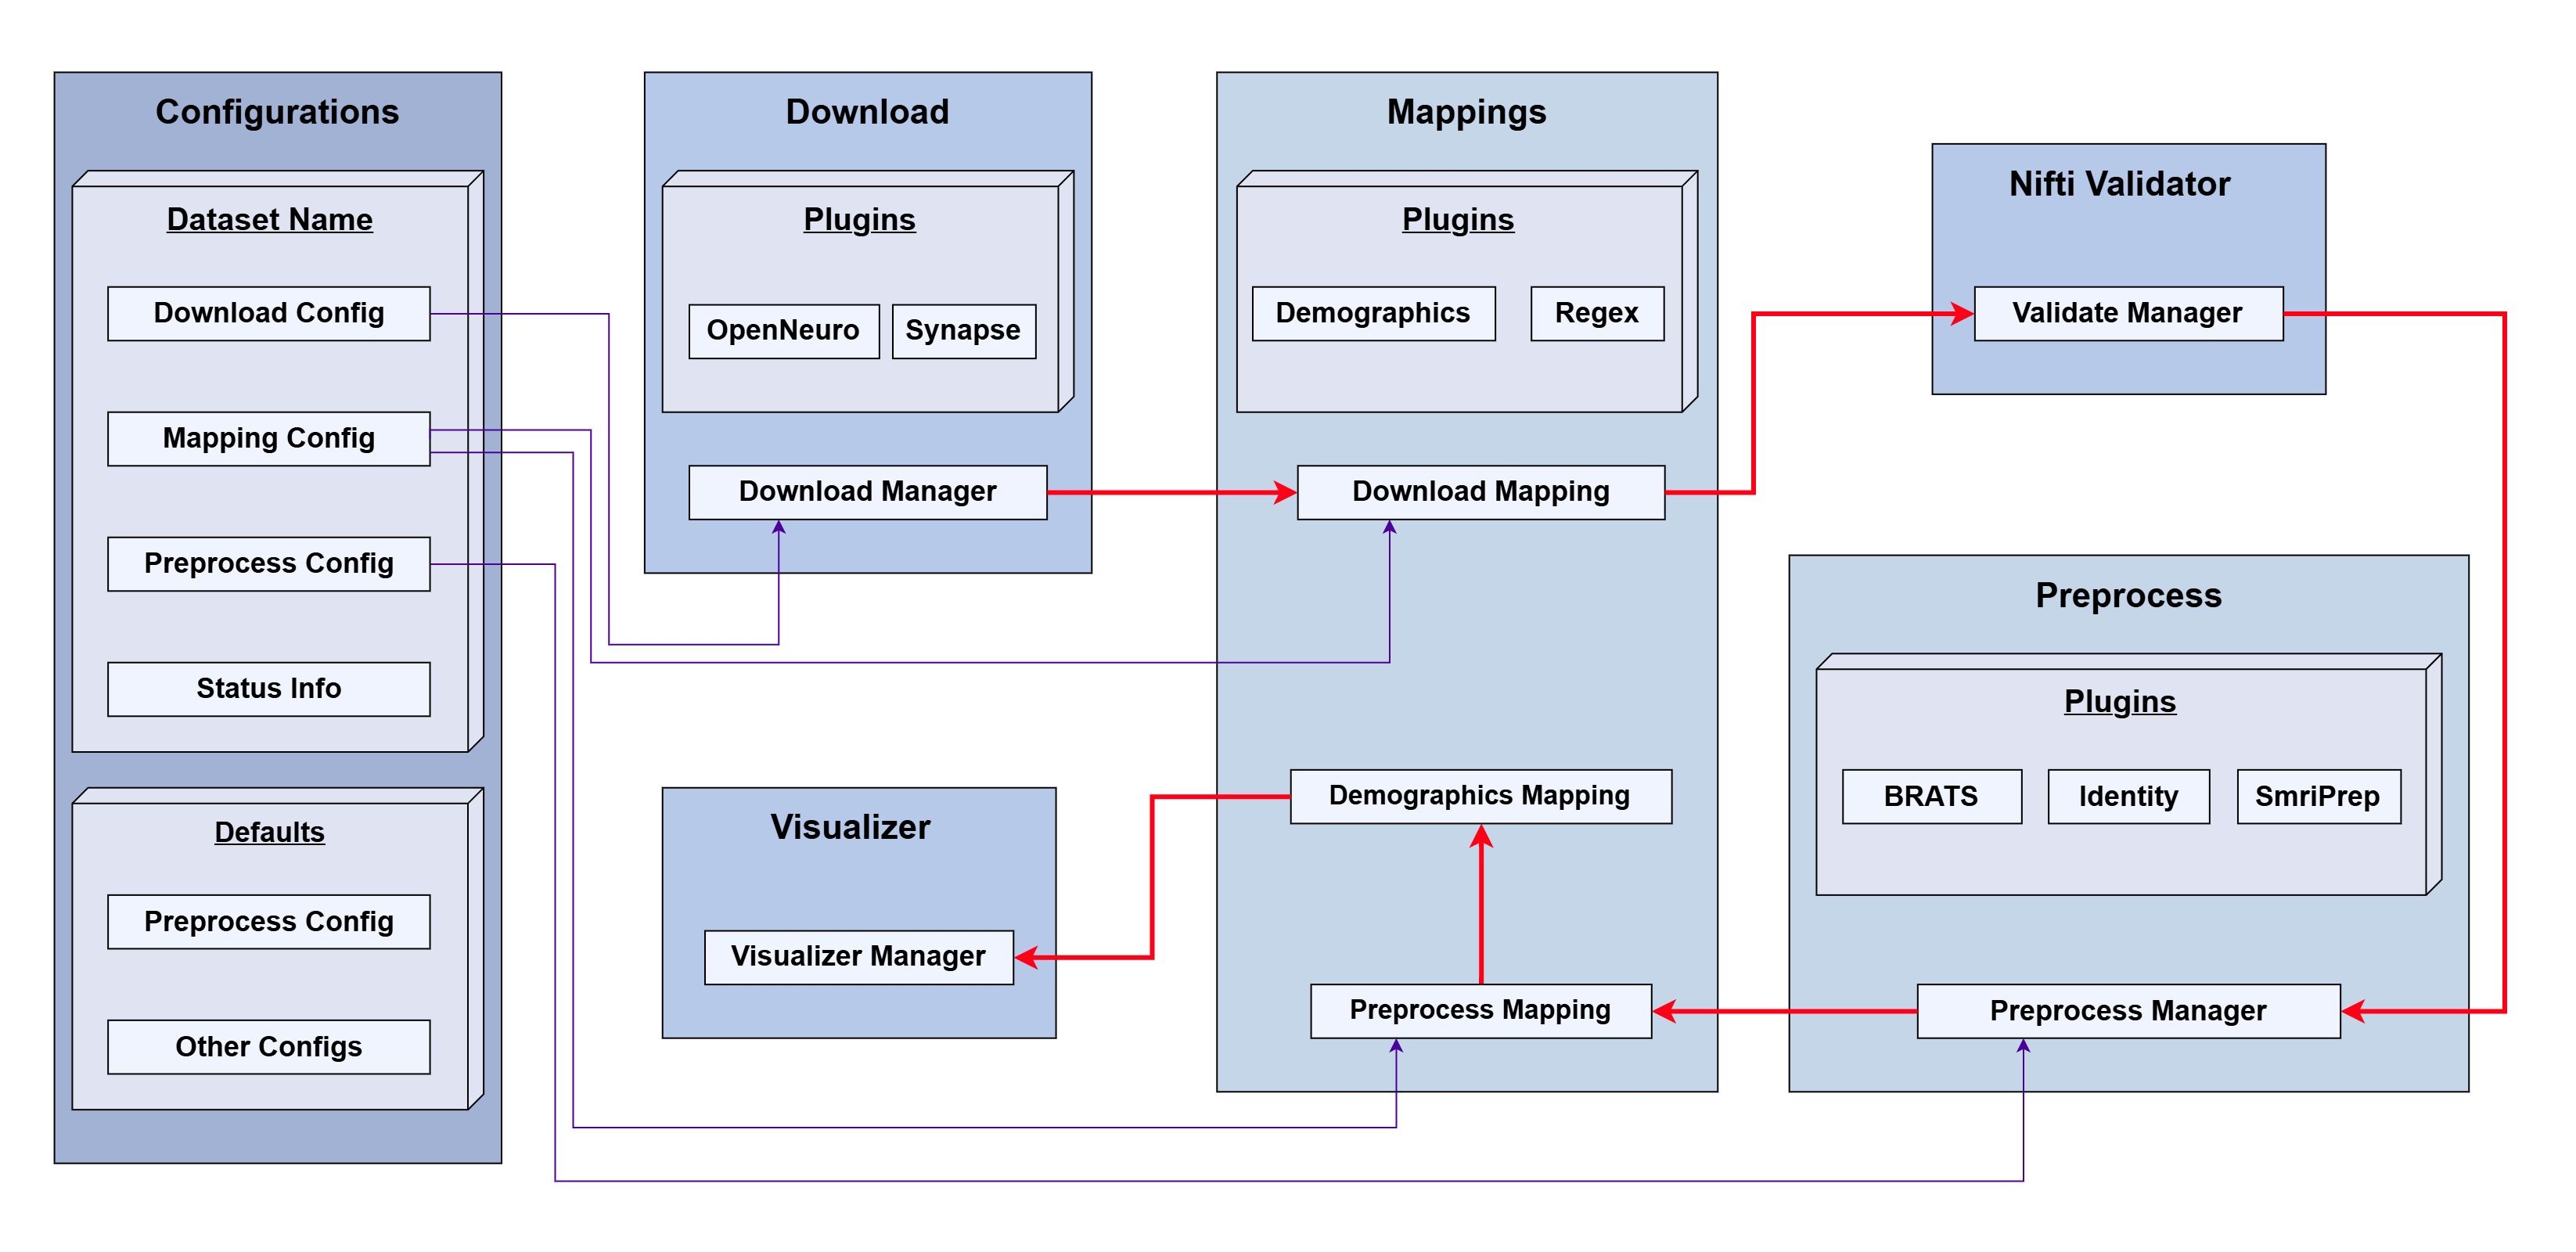
\includegraphics[width=\linewidth]{figures/architecture.png}
    \caption{
        BrainScape Framework architecture.
    }
    \label{fig:SystemArchitecture}\end{center}
\end{figure}

The pipeline workflow coordinates each module's tasks, ensuring a structured flow of data and synchronized processing. 
\textbf{Downloader Plugins}, such as the OpenNeuro downloader and Synapse downloader are used to download MRI 
data from target MRI databases and repositories.
The OpenNeuro downloader uses the \href{https://docs.aws.amazon.com/cli/latest/reference/s3/}{Amazon S3 CLI tool} to download datasets 
from OpenNeuro (\cite{markiewicz2021openneuro}) and other large-scale databases like the Human Connectome Project (HCP) (\cite{van2013wu}).
Similarly, the Synapse Downloader plugin retrieves MRI datasets from \href{https://www.synapse.org}{synapse.org}.
These plugins preserve each downloaded dataset's original folder structure, simplifying comparisons after the datasets are obtained.
\textbf{Mapper Plugins} (e.g., RegexMapper) then map the downloaded dataset files to a standardized JSON record, 
accommodating differences in dataset structure, organization, file formats, and MRI modalities based on user-defined, 
dataset-specific configuration settings.
\textbf{Validator Plugins}, such as the NIfTI Validator, check each MRI file from all of the datasets 
to detect potential errors early, thereby helping the workflow maintain high data-quality standards.

At the next stage of the pipeline, MRI preprocessing is carried out by configurable \textbf{Preprocessor Plugins}, 
each specialized for distinct imaging scenarios and requirements.
Currently, the BrainScape framework supports three primary preprocessing plugins: BraTS, sMRIPrep, and Identity. 
The BraTS preprocessor plugin implements a preprocessing pipeline closely aligned with the well-known 
Brain Tumor Segmentation challenge (BraTS) dataset preprocessing protocol (\cite{menze2014multimodal}) by 
employing the BrainLes-Preprocessing Python package (v0.4.0), publicly available at \url{https://github.com/BrainLesion/preprocessing}. 
This pipeline consists of sequential preprocessing steps, including modality co-registration 
(aligning modalities such as T2-weighted, gadolinium-enhanced T1-weighted (T1Gd), and fluid-attenuated inversion recovery (FLAIR) images to a central T1-weighted modality), 
rigid-body registration to the SRI-24 (\cite{rohlfing2010sri24}) atlas, skull stripping, and intensity normalization. 
The BrainLes-Preprocessing Python package utilizes the Advanced Normalization Tools (ANTs) 
for atlas registration and modality co-registration (\cite{tustison2021antsx}). 
Given the heterogeneous nature of datasets aggregated in BrainScape, 
we implemented a configurable priority-based selection of the central modality, 
with the default priority order set to \texttt{[T1w, T2w, T1Gd, FLAIR]}. 
For brain extraction within the BraTS pipeline, BrainLes-Preprocessing employs ``HD-BET'' (\cite{isensee2019automated}), 
an artificial neural network based tool known for robust, rapid brain extraction across diverse 
clinical MRI sequences (including T1w, T1Gd, T2w, and FLAIR modalities), pathologies, and scanner parameters. 
The HD-BET tool is utilized for brain extraction due to 
its superior accuracy and speed (typically less than 5 seconds per MRI sequence on a GPU) 
compared to widely used tools such as FSL's BET and AFNI's 3dSkullStrip (\cite{isensee2019automated, smith2000bet}).
The sMRIPrep plugin wraps the latest containerized version of the well-established sMRIPrep anatomical MRI preprocessing pipeline (\cite{esteban2021smriprep}), 
openly accessible at \url{https://www.nipreps.org/smriprep/}. 
Within sMRIPrep, anatomical images are aligned using ANTs' antsRegistration algorithm, 
enabling spatial normalization to standard templates such as MNI152 (\cite{avants2008symmetric,avants2011reproducible}).
The BrainScape sMRIPrep plugin runs the latest stable sMRIPrep Docker image (nipreps/smriprep:latest) with its default ANTs-based skull-stripping workflow, 
while disabling FreeSurfer surface reconstruction, Multimodal Surface Matching (MSM), and submillimeter reconstructions 
(\cite{esteban2021smriprep}).
Lastly, the Identity preprocessor plugin serves as a pass-through solution designed explicitly for datasets that 
have already undergone preprocessing or skull stripping. 
This approach ensures previously processed data remain unaltered, significantly simplifying the integration of diverse, 
pre-curated datasets into BrainScape.
For each dataset within the BrainScape dataset collation, 
a dataset-specific configuration file selects the appropriate preprocessing plugin. 
It also supplies all necessary parameters for that plugin, 
enabling each dataset to be preprocessed independently.

All preprocessing plugins currently available handle MRI sessions independently; 
longitudinal pipelines were deliberately omitted because our primary goal is to prepare 
individual T1w, T2w, FLAIR, and T1Gd volumes for downstream deeplearning models.
The sMRIPrep plugin was included because sMRIPrep is one of the most widely used structural MRI preprocessing pipelines, 
while the BraTS and Identity plugins align directly with our subsequent studies on AI-based brain tumour segmentation.
Nevertheless, BrainScape's modular, plugin-based architecture supports the addition of longitudinal or 
other specialized preprocessing pipelines based on the research requirements. 
To facilitate and encourage community-driven extensibility, we provide comprehensive tutorials 
on the BrainScape GitHub repository (\url{https://github.com/yasinzaii/BrainScape}), 
illustrating how researchers can develop custom plugins to meet diverse research requirements.

% \textbf{Preprocessor Plugins} (e.g., BraTS, Identity, sMRIPrep) then employ preprocessing pipelines
% that consist of specialized tasks, such as MRI registration, brain extraction, and intensity normalization. 
% For instance, the BraTS plugin uses the \href{https://github.com/BrainLesion/preprocessing}{BrainLes-Preprocessing} tool, 
% following the Brain Tumor Segmentation (BraTS) pipeline (\cite{menze2014multimodal}). 
% In the BraTS pipeline, multiple MRI modalities are co-registered to a central modality (e.g., T1w), 
% then mapped to the SR24 atlas (\cite{rohlfing2010sri24}), followed by skull stripping and image intensity normalization. 
% Datasets already preprocessed or skull-stripped can opt for simpler pipelines, 
% such as the ``Identity'' preprocessor, which applies no additional operations. 
% Other preprocessing pipelines can also be introduced as needed, maintaining the flexibility and modularity.
After preprocessing, \textbf{Mapper plugins} (e.g., RegexMapper) update the standardized JSON record 
with the preprocessed MRI files. The \textbf{Demographics Mapper} plugin then appends relevant demographic 
and clinical fields (e.g., age, sex, diagnosis) to each subject record, thereby producing a unified 
resource that integrates both anatomical and demographic information.

BrainScape framework's modular, plugin-based architecture supports plugin swaps via configuration files, 
eliminating the need to alter the codebase. As a result, researchers can 
readily include additional plugins supporting specialized pipelines for their unique study requirements. 
BrainScape's pipeline workflow and configurable plugins provide a robust, adaptable system for MRI data management.


\subsection{Experimental Setup and Performance Measurement}

We conducted experiments on a local workstation equipped with a 13th Generation Intel Core i9-13900K CPU 
and an NVIDIA GeForce RTX 4070 Ti GPU (12GB VRAM). 
The CPU has 24 physical cores running at a speed of up to 5.8\,GHz. 
The pipeline was tested using Python 3.11 on Ubuntu 22.04.
To evaluate the BrainScape framework pipeline, 
we selected the publicly available \href{https://openneuro.org/datasets/ds003717}{VASP dataset} (\cite{peelle2022increased}) from OpenNeuro, 
which includes T1w and T2w MRI scans for 60 subjects (120 MRI scans in total). 

We utilized several Python packages to capture performance metrics: 
``time'' for measuring wall-clock time, 
\href{https://docs.python.org/3/library/resource.html}{resource} for computing CPU time,
\href{https://pypi.org/project/psutil/}{psutil} to calculate average CPU utilization, 
\href{https://pypi.org/project/pynvml/}{pynvml} for GPU usage and memory consumption, and 
\href{https://pypi.org/project/codecarbon/}{CodeCarbon} to estimate electricity consumption (kWh) and CO$_2$-equivalents (CO$_2$eq) emissions, 
using the carbon intensity data from New Zealand's local electricity grid.

Currently, the pipeline is designed to process datasets sequentially. 
Nevertheless, its modular design and configurable workflow support running multiple datasets in parallel 
which will be effective in reducing the overall wall-clock time.


\subsection{Hardware and Software Requirements}

BrainScape framework is designed to run on standard 64-bit Linux distributions and has been tested on Ubuntu 22.04. 
Additionally, it supports Windows 10 and 11 through the \href{https://learn.microsoft.com/en-gb/windows/wsl}{Windows Subsystem for Linux 2 (WSL2)}.
Essential software prerequisites include \href{https://www.anaconda.com/docs/getting-started/miniconda/main}{Miniconda} for managing 
a dedicated Python (version 3.11) environment  
and \href{https://docs.aws.amazon.com/cli/latest/userguide/getting-started-install.html}{AWS CLI v2} for accessing and 
downloading MRI data from Amazon S3-hosted repositories, such as \href{https://openneuro.org/}{OpenNeuro}. 
A GPU is recommended to accelerate the computationally intensive preprocessing task of skull stripping 
performed by the HD-BET brain-extraction tool (\cite{isensee2019automated}) in the BraTS plugin. 
However, a GPU is not mandatory; CPU-only systems can still run the pipeline, though they will take longer to preprocess.
Furthermore, BrainScape has been successfully deployed and tested on the 
\href{https://www.nesi.org.nz/}{New Zealand eScience Infrastructure (NeSI)} 
high-performance computing (HPC) platform, demonstrating its scalability and compatibility with cluster computing environments. 
NeSI compute nodes run Rocky Linux, a widely used Red Hat-compatible operating system standard across large-scale HPC facilities. 
Detailed installation instructions, configuration guidelines, and execution documentation are available on
the \href{https://github.com/yasinzaii/BrainScape}{BrainScape GitHub} repository.

